\documentclass[12pt, a4paper, titlepage, table]{article}
\usepackage{pdfpages}
\usepackage[utf8]{inputenc}
\usepackage[T1]{fontenc}
\usepackage{titlesec}
\usepackage[french]{babel}
\usepackage{caption}
\usepackage{float}
\usepackage{graphicx}
\usepackage[inner=2cm, outer=2cm, top=2cm, bottom=2cm]{geometry}
\usepackage[T1]{fontenc}
\usepackage{times}
\usepackage{xr} 
\usepackage{multirow}
\usepackage{amsmath}
\usepackage{array}
\usepackage{booktabs}
\usepackage{tabularx}
\usepackage{ragged2e}
\usepackage{adjustbox}

\begin{document}
	\label{document}
	\title{Etude de l'insertion professionnelle des diplômés de l'université (DUT, Licence Pro, MASTER LMD et Master ENS)}
	\author{Sébastien Mertès}
	\date{\today}
	\maketitle
	\renewcommand{\thesection}{\arabic{section}.}
	\renewcommand{\thesubsection}{\thesection\arabic{subsection}}
	\renewcommand{\tablename}{Tableau}
	\renewcommand{\abstractname}{Résumé}
	\captionsetup[table]{font={small}}
	\setlength{\parindent}{0pt}
	\captionsetup{labelfont=bf, font=small}
	\tableofcontents
	\newcolumntype{C}{>{\RaggedRight\arraybackslash}X}
	\newpage
	
\section{Introduction}
	
\section{Présentation des données}
	Nous avons 3 jeux de données représentant respectivement les informations concernant l'évaluation de l'insertion professionnelle sur le marché du travail des diplômés universitaires en DUT, Licence Professionnelle, Master LMD (Licence-Master-Doctorat) et Master ENS (Enseignement) de toutes les disciplines. 
	
	Ces données ont été collectées 18 mois et 30 mois après l'obtention du diplôme des sessions  2013 à 2019. Ainsi l'enquête a commencé en décembre 2015, pour s'achever en décembre 2021.
	
	Les données collectées regroupent, par niveau de diplôme, les disciplines, le taux d'insertion, le salaire brut et net estimé, le pourcentage des types de contrat professionnel (CDI, CDD, intérimaire etc...) ainsi que les secteurs d'activité, les professions et le type d'entreprises.
	
	Les tableaux 1 à 5 décrivent les différentes variables utilisées pour cette étude et le taux en pourcentage de valeurs manquantes de chaque modalité pour les les différentes catégories.
	
	Le Tableaux 1, présente la liste des diplômes universitaires pour les DUT, Licence Professionnelle et MASTERS.
	Les MASTERS sont distingués par le MASTER LMD et le MASTER ENS. 
	
	Les disciplines sont indiquées aussi bien individuellement (Informatique, histoire, droit, psychologie etc..), que par des ensembles de disciplines (Formations juridiques, économiques et de gestion, Sciences humaines et sociales etc...). L'ensemble de toutes les disciplines par niveau de diplôme est aussi indiqué (Ensemble MASTERS LMD, Ensemble des départements d'IUT etc...).   
	
	
	
\newpage

\begin{table}[H]
	\centering
	\begin{adjustbox}{max width=\textwidth}
		\begin{tabularx}{\linewidth}{|l|C|}
			\hline
			\multicolumn{1}{|c|}{\textbf{Diplôme}} & \multicolumn{1}{c|}{\textbf{Définition}} \\
			\hline
			DUT & Diplôme Universitaire de Technologie. Formation de 2 ans axée sur des compétences techniques et pratiques. \\
			\hline
			LICENCE PRO & Licence professionnelle. Programme de 1 an après un DUT ou une Licence, offrant une spécialisation professionnelle. \\
			\hline
			MASTER ENS & Master Enseignement. Diplôme permettant de devenir enseignant dans le système éducatif français. \\
			\hline
			MASTER LMD & Système européen d'enseignement supérieur avec niveaux de Licence, Master et Doctorat. \\
			\hline
		\end{tabularx}
	\end{adjustbox}
	\caption{Nom de la variable catégorielle et ses modalités concernant les diplômes universitaires}
	\label{tab:diplomes}
\end{table}

\begin{table}[H]
	\centering
	\begin{adjustbox}{max width=\textwidth}
	\begin{tabularx}{\linewidth}{|l|C|}
		\hline
		\multicolumn{1}{|c|}{\textbf{Discipline}} & \multicolumn{1}{c|}{\textbf{Ensemble}} \\
		\hline
		Autres sciences humaines et sociales & Ensemble Licence professionnelle \\
		\hline
		Autres formations juridiques, économiques et de gestion & Ensemble formations juridiques, économiques et de gestion \\
		\hline
		Sciences de la vie et de la terre & Ensemble des départements d'IUT \\
		\hline
		Psychologie & Ensemble sciences humaines et sociales \\
		\hline
		Information communication & Ensemble sciences, technologies et santé \\
		\hline
		Lettres, langues, arts & Autres sciences, technologies et santé \\
		\hline
		Sciences de l'ingénieur & Ensemble Masters LMD (hors Masters enseignement et hors Dauphine et Antilles-Guyane) \\
		\hline
		Histoire-géographie & Ensemble Masters LMD (hors Masters enseignement) \\
		\hline
		Droit & \\
		\hline
		Informatique & \\
		\hline
		Gestion & \\
		\hline
		Sciences fondamentales & \\
		\hline
		Économie & \\
		\hline
		Masters enseignement & \\
		\hline
	\end{tabularx}
	\end{adjustbox}
	\caption{Liste des disciplines et ensembles}
	\label{tab:disciplines}
\end{table}


\begin{table}[H]
	\centering
	\begin{tabularx}{\textwidth}{|X|c|}
		\hline
		\textbf{Contrat} & \textbf{\%} \\
		\hline
		Prof. libérale, indépendant, chef d’entreprise & 8.1 \\
		\hline
		Fonctionnaire & 8.1 \\
		\hline
		CDI & 8.1 \\
		\hline
		CDI de chantier ou CDI de mission & 8.8 \\
		\hline
		Contrat spécifique au doctorat & 10.5 \\
		\hline
		CDD & 8.1 \\
		\hline
		Vacataire & 8.1 \\
		\hline
		Intérimaire & 8.1 \\
		\hline
		Intermittent du spectacle & 8.1 \\
		\hline
		Contrat de professionnalisation & 8.1 \\
		\hline
		Emplois aidés (Contrat Initiative Emploi…) & 8.1 \\
		\hline
		Volontariat international & 8.1 \\
		\hline
	\end{tabularx}
	\caption{Pourcentage de valeurs manquantes des différents types de contrat}
	\label{tab:contrats_pourcentage}
\end{table}

\begin{table}[H]
	\centering
	\begin{tabularx}{\textwidth}{|X|c|}
		\hline
		\textbf{Entreprise} & \textbf{\%} \\
		\hline
		Vous-même & 11.0 \\
		\hline
		La fonction publique (d'etat, territoriale ou hospitalière) & 11.0 \\
		\hline
		Une entreprise privée & 11.0 \\
		\hline
		Une entreprise publique & 11.0 \\
		\hline
		Une association & 11.0 \\
		\hline
		Une personne exerçant une profession libérale ou un indépendant & 11.0 \\
		\hline
		Organisation internationale ou une institution de l'Union européenne & 11.5 \\
		\hline
		Société d'économie mixte & 11.4 \\
		\hline
		Un particulier & 11.0 \\
		\hline
	\end{tabularx}
	\caption{Pourcentage de valeurs manquantes par type d'entreprise}
	\label{tab:entreprise_pourcentage}
\end{table}


\begin{table}[H]
	\centering
	\begin{tabularx}{\textwidth}{|X|c|}
		\hline
		\textbf{Secteur} & \textbf{\%} \\
		\hline
		Agriculture, sylviculture et pêche & 7.1 \\
		\hline
		Industries (manufacturières, extractives et autres) & 7.1 \\
		\hline
		Construction & 7.1 \\
		\hline
		Activités immobilières & 7.4 \\
		\hline
		Commerce, transports, hébergement et restauration & 7.1 \\
		\hline
		Information et communication & 7.1 \\
		\hline
		Activités financières et d’assurance & 7.1 \\
		\hline
		Activités spécialisées, scientifiques et techniques & 7.1 \\
		\hline
		Activités de services administratifs et de soutien & 7.1 \\
		\hline
		Enseignement & 7.1 \\
		\hline
		Administration publique (hors enseignement) & 7.1 \\
		\hline
		Santé humaine et action sociale & 7.1 \\
		\hline
		Arts, spectacles et activités récréatives & 7.1 \\
		\hline
		Autres activités de service & 7.1 \\
		\hline
	\end{tabularx}
	\caption{Pourcentage de valeurs manquantes par secteur}
	\label{tab:secteurs_pourcentage}
\end{table}

\begin{table}[H]
	\centering
	\begin{tabularx}{\textwidth}{|X|c|}
		\hline
		\textbf{Profession} & \textbf{\%} \\
		\hline
		Agriculteur & 11.2 \\
		\hline
		Artisan, commerçant, chef d'entreprise & 11.1 \\
		\hline
		Profession libérale & 11.1 \\
		\hline
		Personnel de catégorie A de la fonction publique & 10.2 \\
		\hline
		Ingénieur, cadre, professions libérales, professions intellectuelles supérieures & 10.2 \\
		\hline
		Personnel de catégorie B de la fonction publique & 10.2 \\
		\hline
		Emploi de niveau intermédiaire : technicien, agent de maîtrise, etc. & 10.2 \\
		\hline
		Personnel de catégorie C de la fonction publique & 10.2 \\
		\hline
		Manœuvre, ouvrier & 10.2 \\
		\hline
		Employé de bureau, de commerce, personnel de service & 5.3 \\
		\hline
	\end{tabularx}
	\caption{Pourcentage de valeurs manquantes par profession}
	\label{tab:professions_pourcentage}
\end{table}


\section{Les types de contrats après l'obtention du diplôme}

	\subsection{Répartion des contrats à 18 et 30 mois après l'obtention du diplôme}
		\begin{figure}[H]
			\centering
			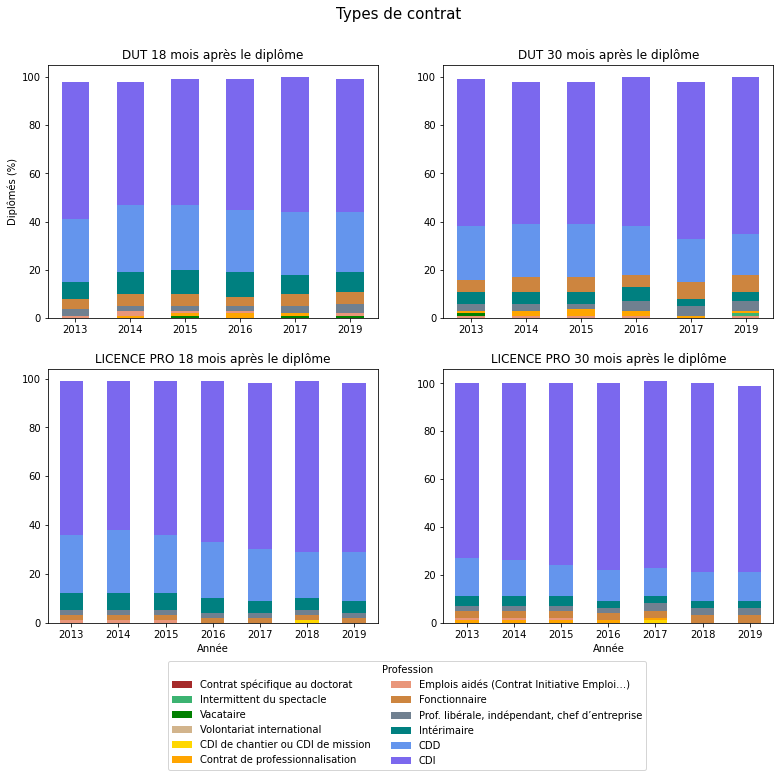
\includegraphics[width=1\textwidth]{../graphs/repartition_contrats_situation_1.png}
			\captionof{figure}{Répartition des contrats à 18 et 30 mois après l'obtention du diplôme}
			\label{fig:contrat_pourcentage_1}
		\end{figure}
	
		\begin{figure}[H]
			\centering
			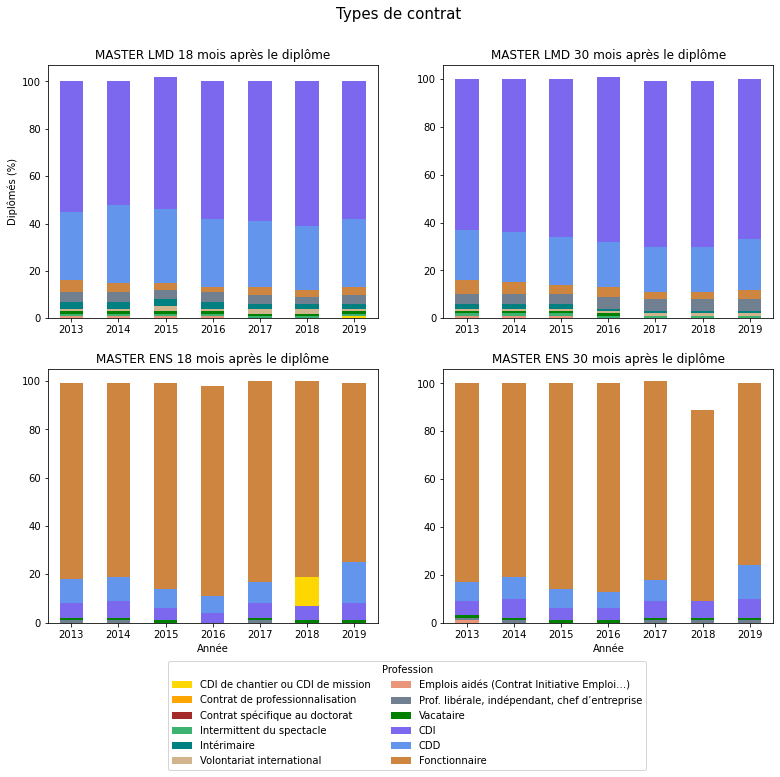
\includegraphics[width=1\textwidth]{../graphs/repartition_contrats_situation_2.png}
			\captionof{figure}{Répartition des contrats à 18 et 30 mois après l'obtention du diplôme}
			\label{fig:contrat_pourcentage_2}
		\end{figure}

\section{Les professions après l'obtention du diplôme}

	\subsection{Répartition des professions à 18 et 30 mois après l'obtention du diplôme}
		\begin{figure}[H]
			\centering
			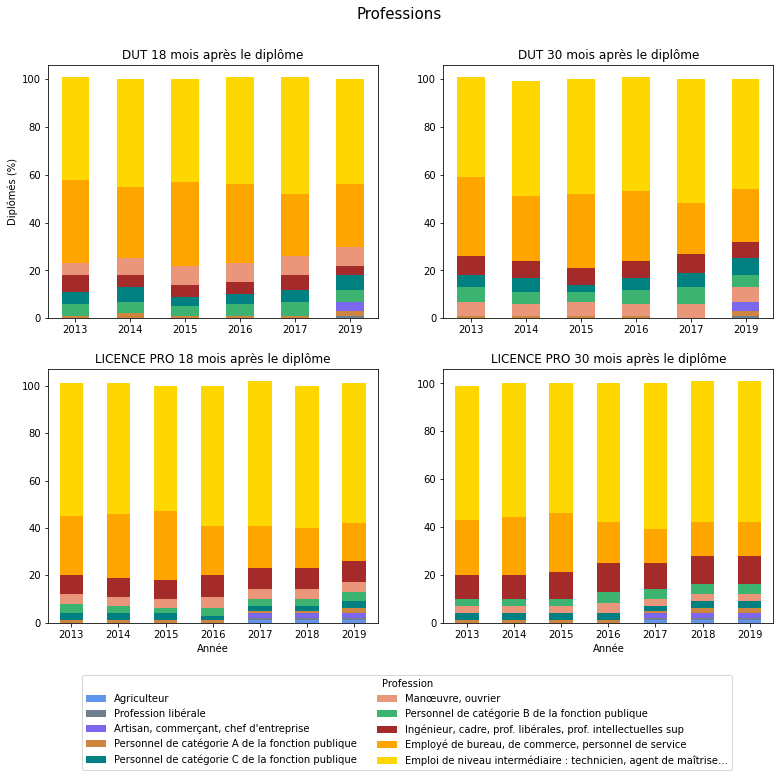
\includegraphics[width=1\textwidth]{../graphs/repartition_professions_situation_1.png}
			\captionof{figure}{Répartition des professions à 18 et 30 mois après l'obtention du diplôme (DUT-Licence pro)}
			\label{fig:profession_pourcentage_1}
		\end{figure}
	
		\begin{figure}[H]
			\centering
			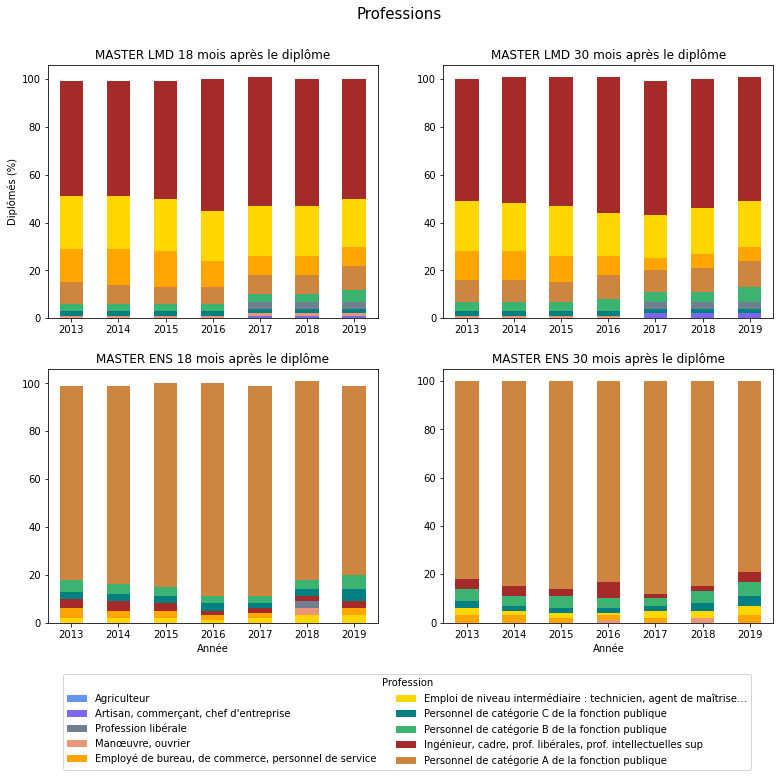
\includegraphics[width=1\textwidth]{../graphs/repartition_professions_situation_2.png}
			\captionof{figure}{Répartition des professions à 18 et 30 mois après l'obtention du diplôme (Masters)}
			\label{fig:profession_pourcentage_2}
		\end{figure}


\section{Secteurs d'activité après l'obtention du diplôme}
	Les données 18 mois après l'obtention du diplôme étant manquantes, nous indiquons dans la Figure 5, le pourcentage des secteurs d'activité dans lesquels les diplômés se sont insérés 30 mois après son obtention. 

	\begin{figure}[H]
		\centering
		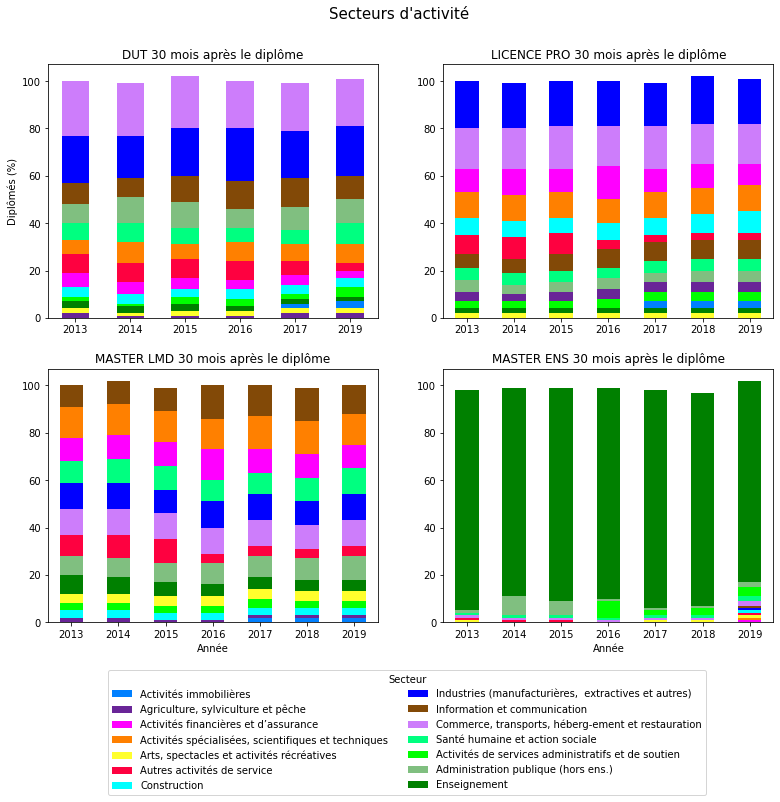
\includegraphics[width=1\textwidth]{../graphs/repartition_secteurs_situation.png}
		\captionof{figure}{Répartition des secteurs à 18 et 30 mois après l'obtention du diplôme}
	\end{figure}

\section{Proportion des diplômés et des diplômes universitaires}

	\subsection{Proportion des diplômés}
	Le Tableau \ref{tab:genre_responses} et la Figure \ref{fig:genre_reponses} fournissent la proportion des hommes et des femmes de l'ensemble des diplômés de 2013 à 2019 ayant répondu à l'enquête. Ainsi nous avons environ 12 \% de réponses à l'enquête en plus de la part des femmes par rapport au hommes, pourtant à un total d'environ 665000 de diplômés interrogés.
		\begin{table}[H]
			\centering
			\begin{tabular}{lcc}
				\toprule
				\textbf{Genre} & \textbf{Diplômé} & \textbf{\%} \\
				\midrule
				Femmes & 371350 & 55.85 \\
				Hommes & 293586 & 44.15 \\
				\bottomrule
			\end{tabular}
			\caption{Nombre et proportion de diplômés par genre (2013 à 2019)}
			\label{tab:genre_responses}
		\end{table}
	
		\begin{figure}[H]
			\centering
			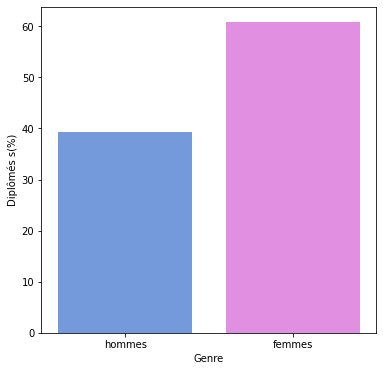
\includegraphics[width=0.6\textwidth]{../graphs/proportion_genre.png}
			\captionof{figure}{Proportion des diplômés selon genre (2013 à 2019)}
			\label{fig:genre_reponses}
		\end{figure}
	
	\subsection{Proportion des diplômes universitaire}
	Le Tableau \ref{tab:diplome_genre} et la Figure \ref{fig:diplome_genre} présentent le nombre et la proportion de diplômés par niveau de diplôme universitaire selon le genre. 
		\begin{table}[H]
			\centering
			\begin{tabular}{lllc}
				\toprule
				\textbf{Diplôme} & \textbf{Genre} & \textbf{Diplômé} & \textbf{\%} \\
				\midrule
				DUT & Femmes & 9166 & 1.4 \\
				DUT & Hommes & 15218 & 2.3 \\
				LICENCE PRO & Femmes & 83290 & 12.5 \\
				LICENCE PRO & Hommes & 111794 & 16.8 \\
				MASTER ENS & Femmes & 56912 & 8.6 \\
				MASTER ENS & Hommes & 16400 & 2.5 \\
				MASTER LMD & Femmes & 221982 & 33.4 \\
				MASTER LMD & Hommes & 150174 & 22.6 \\
				\bottomrule
			\end{tabular}
			\caption{Nombre et proportion (\%) de diplômés par diplôme selon le genre (2013 à 2019)}
			\label{tab:diplome_genre}
		\end{table}
	Nous constatons que les diplômés de la filière des DUT sont largement moins représentés que ceux des licences professionnelles et des masters LMD. Il y a également moins de diplômés dans l'enquête pour le Master ENS avec une proportion plus forte de 6.1 \% de femmes par rapport aux hommes.
	Les Licences professionnelles et les Masters LMD rassemblent la majorité des diplômés de l'enquête avec 29,3 \% pour les licences pro et 56 \% pour les Masters LMD.
	Nous constatons que les femmes représentent la majorité des diplômés en Masters. Les hommes représentent environ 19 \% des diplômés en DUT et Licences professionnelles contre 13.9 \% pour les femmes. Mais les femmes représentent 42 \% des diplômés en Masters qui ont répondu à l'enquête contre 31.2 \% pour les hommes.
		\begin{figure}[H]
			\centering
			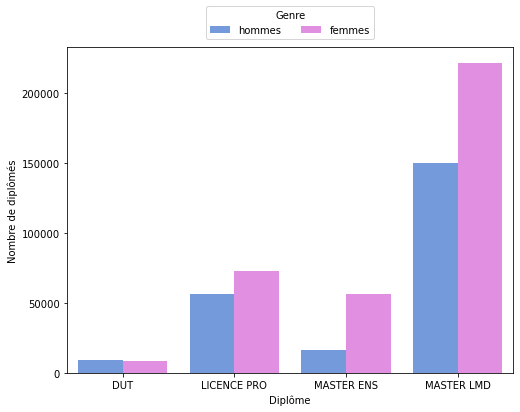
\includegraphics[width=0.8\textwidth]{../graphs/nombre_diplome_genre.png}
			\captionof{figure}{Nombre de diplômés par diplôme selon le genre (2013 à 2019)}
			\label{fig:diplome_genre}
		\end{figure}
	
	La plus forte proportion de femmes dans les filières plus longues (Masters) par rapport aux hommes est-elle liée au nombre insuffisant de réponses à l'enquête s'agissant des hommes ( -12 \% / femmes) ou bien les femmes sont-elles plus en capacité de choisir des études plus longues et moins techniques que leurs homologues masculins ?
	
	Il semblerait, dans l'hypothèse d'un effectif constant pour les femmes, que même avec 12 \% de diplômés masculins en plus, il serait difficile de rattraper les effectifs des femmes en Masters puisque le différentiel de diplômés est déjà d'environ 11 \% en faveur des femmes.      

\section{Proportion des disciplines des diplômés}
	\begin{table}[H]
		\centering
		\begin{tabular}{lllc}
			\toprule
			\textbf{Genre} & \textbf{Discipline} & \textbf{Diplômé} & \textbf{\%} \\
			\midrule
			Hommes & Sciences de l'ingénieur & 80980.0 & 12.2 \\
			& Gestion & 59674.0 & 9.0 \\
			& Informatique & 33584.0 & 5.1 \\
			& Sciences de la vie et de la terre & 25126.0 & 3.8 \\
			& Lettres, langues, arts & 16652.0 & 2.5 \\
			& Masters enseignement & 16400.0 & 2.5 \\
			& Sciences fondamentales & 16338.0 & 2.5 \\
			& Droit & 13818.0 & 2.1 \\
			& Économie & 11840.0 & 1.8 \\
			& Information communication & 9758.0 & 1.5 \\
			& Histoire-géographie & 7180.0 & 1.1 \\
			& Psychologie & 2236.0 & 0.3 \\
			\midrule
			Femmes & Gestion & 83264.0 & 12.5 \\
			& Lettres, langues, arts & 58158.0 & 8.7 \\
			& Masters enseignement & 56912.0 & 8.6 \\
			& Sciences de la vie et de la terre & 40958.0 & 6.2 \\
			& Droit & 31676.0 & 4.8 \\
			& Information communication & 20006.0 & 3.0 \\
			& Sciences de l'ingénieur & 16914.0 & 2.5 \\
			& Sciences fondamentales & 16264.0 & 2.4 \\
			& Psychologie & 15898.0 & 2.4 \\
			& Économie & 15334.0 & 2.3 \\
			& Histoire-géographie & 11228.0 & 1.7 \\
			& Informatique & 4738.0 & 0.7 \\
			\bottomrule
		\end{tabular}
		\caption{Nombre et proportion (\%) des disciplines des diplômés selon le genre (2013 à 2019)}
		\label{tab:genre_discipline}
	\end{table}
	Le Tableau \ref{tab:genre_discipline} et la Figure \ref{fig:genre_discipline} présentent le nombre de diplômés par discipline ainsi que leur proportion (\%) par rapport à l'ensemble des diplômés ayant répondu à l'enquête.
	Nous constatons, entre les hommes et les femmes,  une nette inversion de la proportion des disciplines  littéraires (8,7 \% contre 2,5 \%) ou de gestion et comptabilité (12,5 \% contre 9 \%) ou dans l'enseignement (8,6 \% contre 2,5 \%) par rapport aux domaines plus techniques et scientifiques comme les sciences de l'ingénieur (12,2 \% contre 2,5 \%) ou encore l'informatique (5.1 \% contre 0,7 \%)

	\begin{figure}[H]
		\centering
		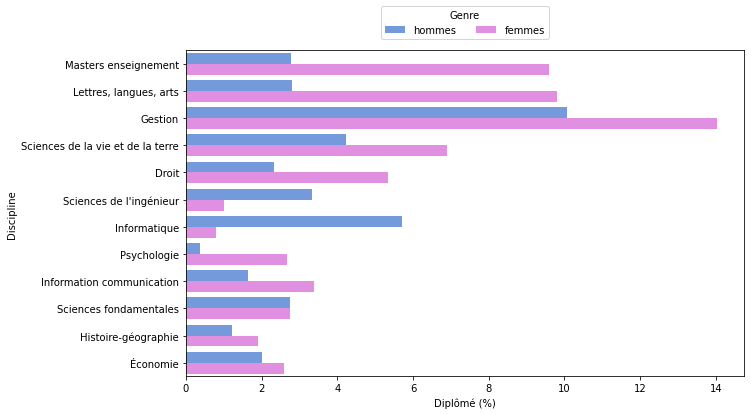
\includegraphics[width=1\textwidth]{../graphs/proportion_disciplines.png}
		\captionof{figure}{Proportion (\%) des disciplines des diplômés selon le genre (2013 à 2019)}
		\label{fig:genre_discipline}
	\end{figure}

	La remarque précédente conduisant à soumettre l'hypothèse que les femmes choisiraient majoritairement les filières universitaires les plus longues (Masters) serait confirmée par les disciplines choisies.
	En effet, les domaines de l'enseignement ou encore littéraires sont des domaines dont les années d'études sont les plus longues pour aboutir à une insertion professionnelle plus prometteuse.
	Alors que les hommes préféraient davantage une insertion plus rapide sur le marché du travail en choisissant l'ingénierie (12,2 \% contre 2.5 \%), davantage corrélée à l'industrie ou encore en filières plus courtes, les licences professionnelles (16,8 \% contre 12,5 \%). 

\section{Taux d'insertion des diplômés dans les emplois stables}

Le taux d’insertion est défini comme étant le pourcentage de diplômés occupant un emploi, quel qu’il soit, sur l’ensemble des diplômés présents sur le marché du travail. Il est calculé sur les diplômés de nationalité française, issus de la formation initiale, entrés immédiatement et durablement sur le marché du travail après l’obtention de leur diplôme en 2013, 2014, 2015, 2016, 2017, 2018 ou 2019.


\section{La question épineuse des salaires}
L’information collectée sur le salaire porte sur le salaire net, primes comprises. Les salaires affichés correspondent aux valeurs médianes sur les emplois à temps plein. A partir de ces valeurs, on estime un salaire brut annuel, sur la base d’un taux forfaitaire de passage du net au brut de 1,3 (donnée moyenne constatée sur les salaires du secteur privé).

	\subsection{Salaires médians}

	Le Tableau \ref{tab:salaire_median_genre} et la Figure \ref{fig:salaire_median_genre} montrent le salaire net mensuel médian des emplois stables entre les hommes et les femmes. 

	\begin{table}[H]
		\centering
		\begin{tabular}{llr}
			\toprule
			\textbf{Genre} & \textbf{Diplôme} & \textbf{{Salaire net mensuel médian (€)}} \\
			\midrule
			Femmes & Master LMD & 1760 \\
			& Master ENS & 1750 \\
			& Licence PRO & 1520 \\
			& DUT & 1410 \\
			\midrule
			Hommes & Master LMD & 2000 \\
			& Master ENS & 1800 \\
			& Licence PRO & 1670 \\
			& DUT & 1600 \\
			\bottomrule
		\end{tabular}
		\caption{Salaire net mensuel médian des emplois à temps plein par genre et diplôme}
		\label{tab:salaire_median_genre}
	\end{table}
	
	Nous observons que les hommes ont un salaire médian plus élevé d'environ quelques soit leur niveau de diplôme.
	Sans surprise, plus le niveau d'étude des diplômés est élevé et plus les salaires sont élevés.
	Les hommes diplômés au niveau Master aurait un salaire médian de 200 € plus élevé que celui des femmes avec le même niveau d'études.
	Nous remarquons que pour le Master enseignement (ENS) le salaire médian est pratiquement équivalent.  
	La Figure \ref{fig:contrat_pourcentage_2} nous apprend qu'au niveau des Masters ENS l'essentiel des diplômés sont dans la fonction publique contraire au Masters LMD qui sont essentiellement dans le secteur privé.
	Cela supposerait que les hommes choisissant majoritairement des filière 
	
		
	\begin{figure}[H]
		\centering
		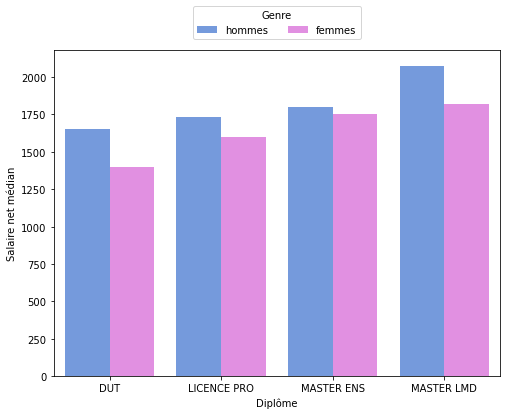
\includegraphics[width=0.7\textwidth]{../graphs/salaires_medians_genre.png}
		\captionof{figure}{Salaire net mensuel médian par genre des emplois stables(€) (2013 à 2019)}
		\label{fig:salaire_median_genre}
	\end{figure}
	Cela supposerait que les hommes choisissant majoritairement les filières dans l’ingénierie ou encore l'informatique auraient par la discipline et le secteur privé des salaires plus élevés que les femmes au même niveau d'études mais choisissant des disciplines moins rémunératrices (Gestion, littéraires, enseignement, etc..). 

\end{document}